\documentclass[../documentation.tex]{subfiles}

\begin{document}

\thispagestyle{empty} % no page number

\subsection{Initial Gantt chart}

I chose the waterfall Gantt chart to plan the actions
throughout the project.

\begin{figure}[h]
    \centering
    \makebox[\textwidth][c]{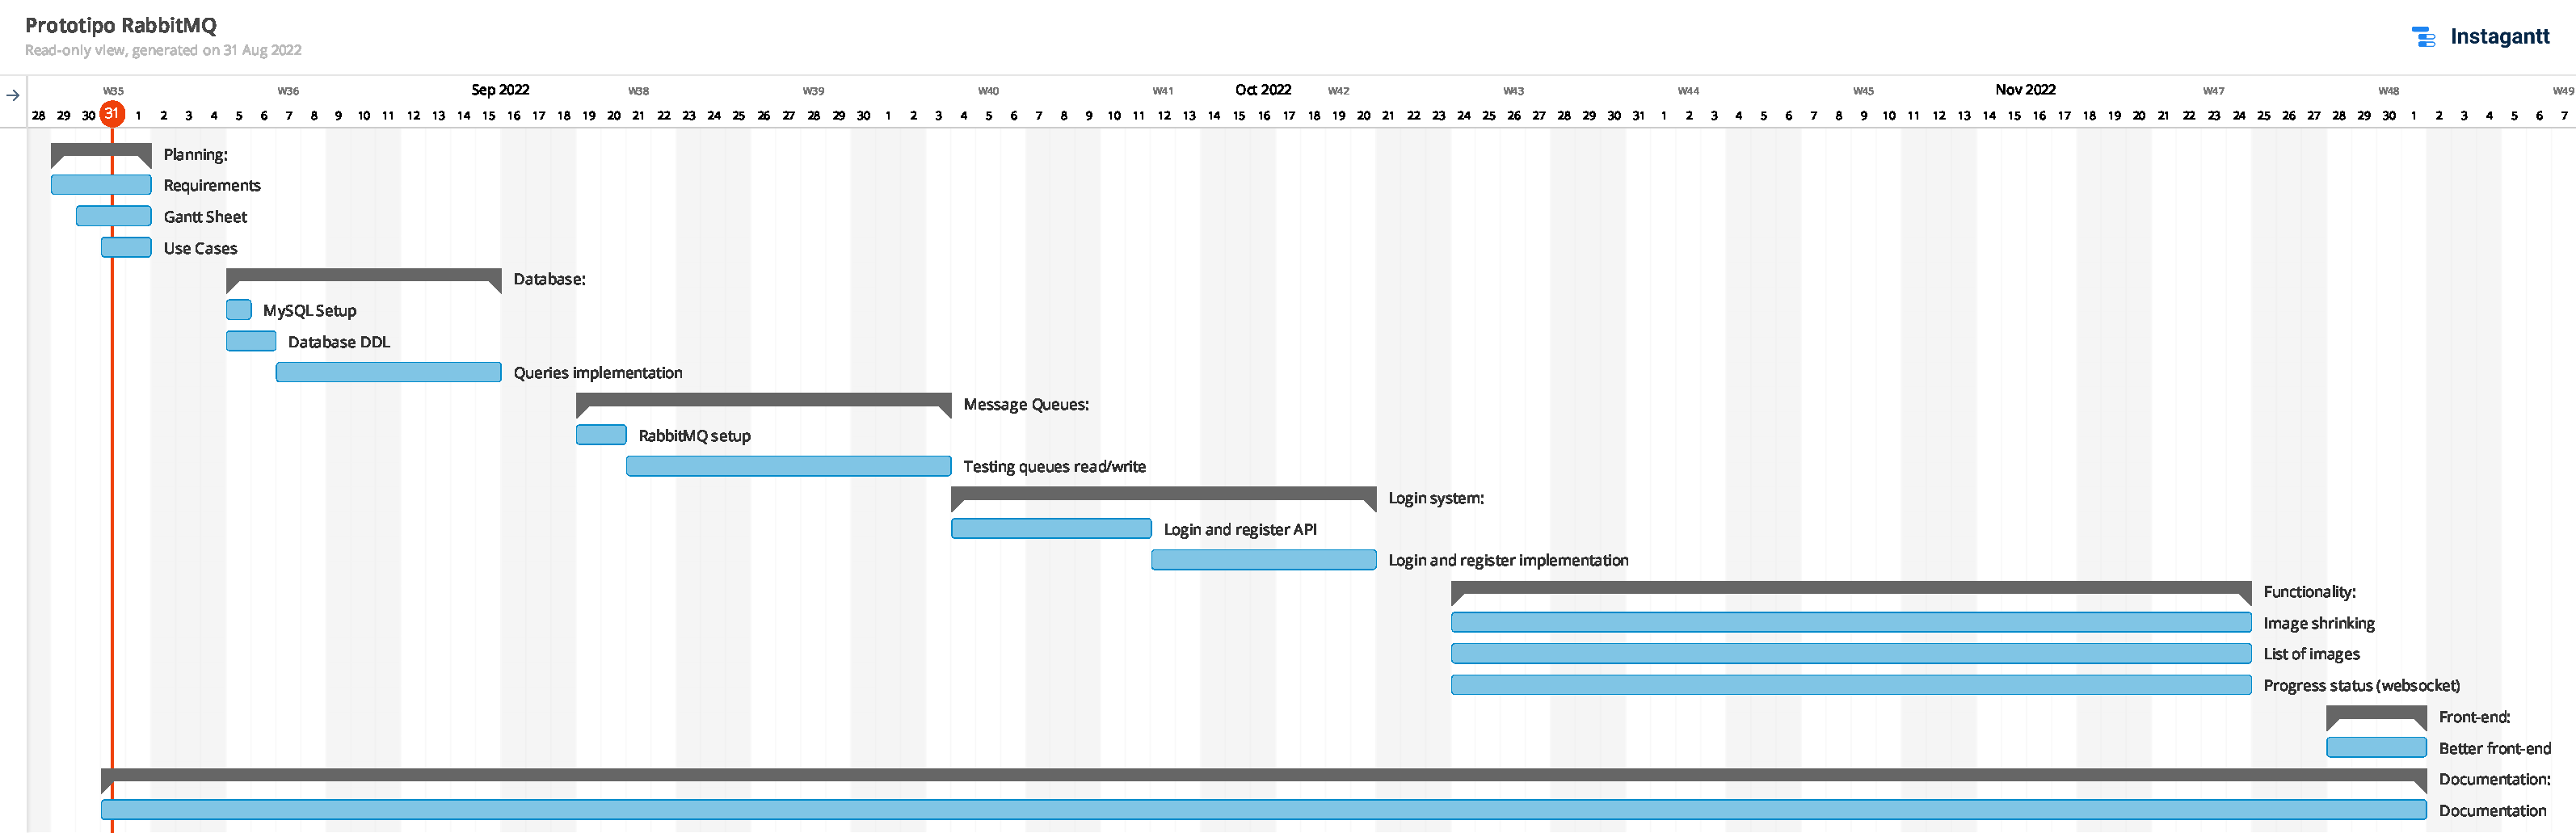
\includegraphics[width=1.3\pagewidth]{gantt1.pdf}}%
    \caption{Initial Gantt chart}
\end{figure}

\pagebreak

\thispagestyle{empty} % no page number
            
\subsection{Final Gantt chart}

\begin{figure}[h]
    \centering
    \makebox[\textwidth][c]{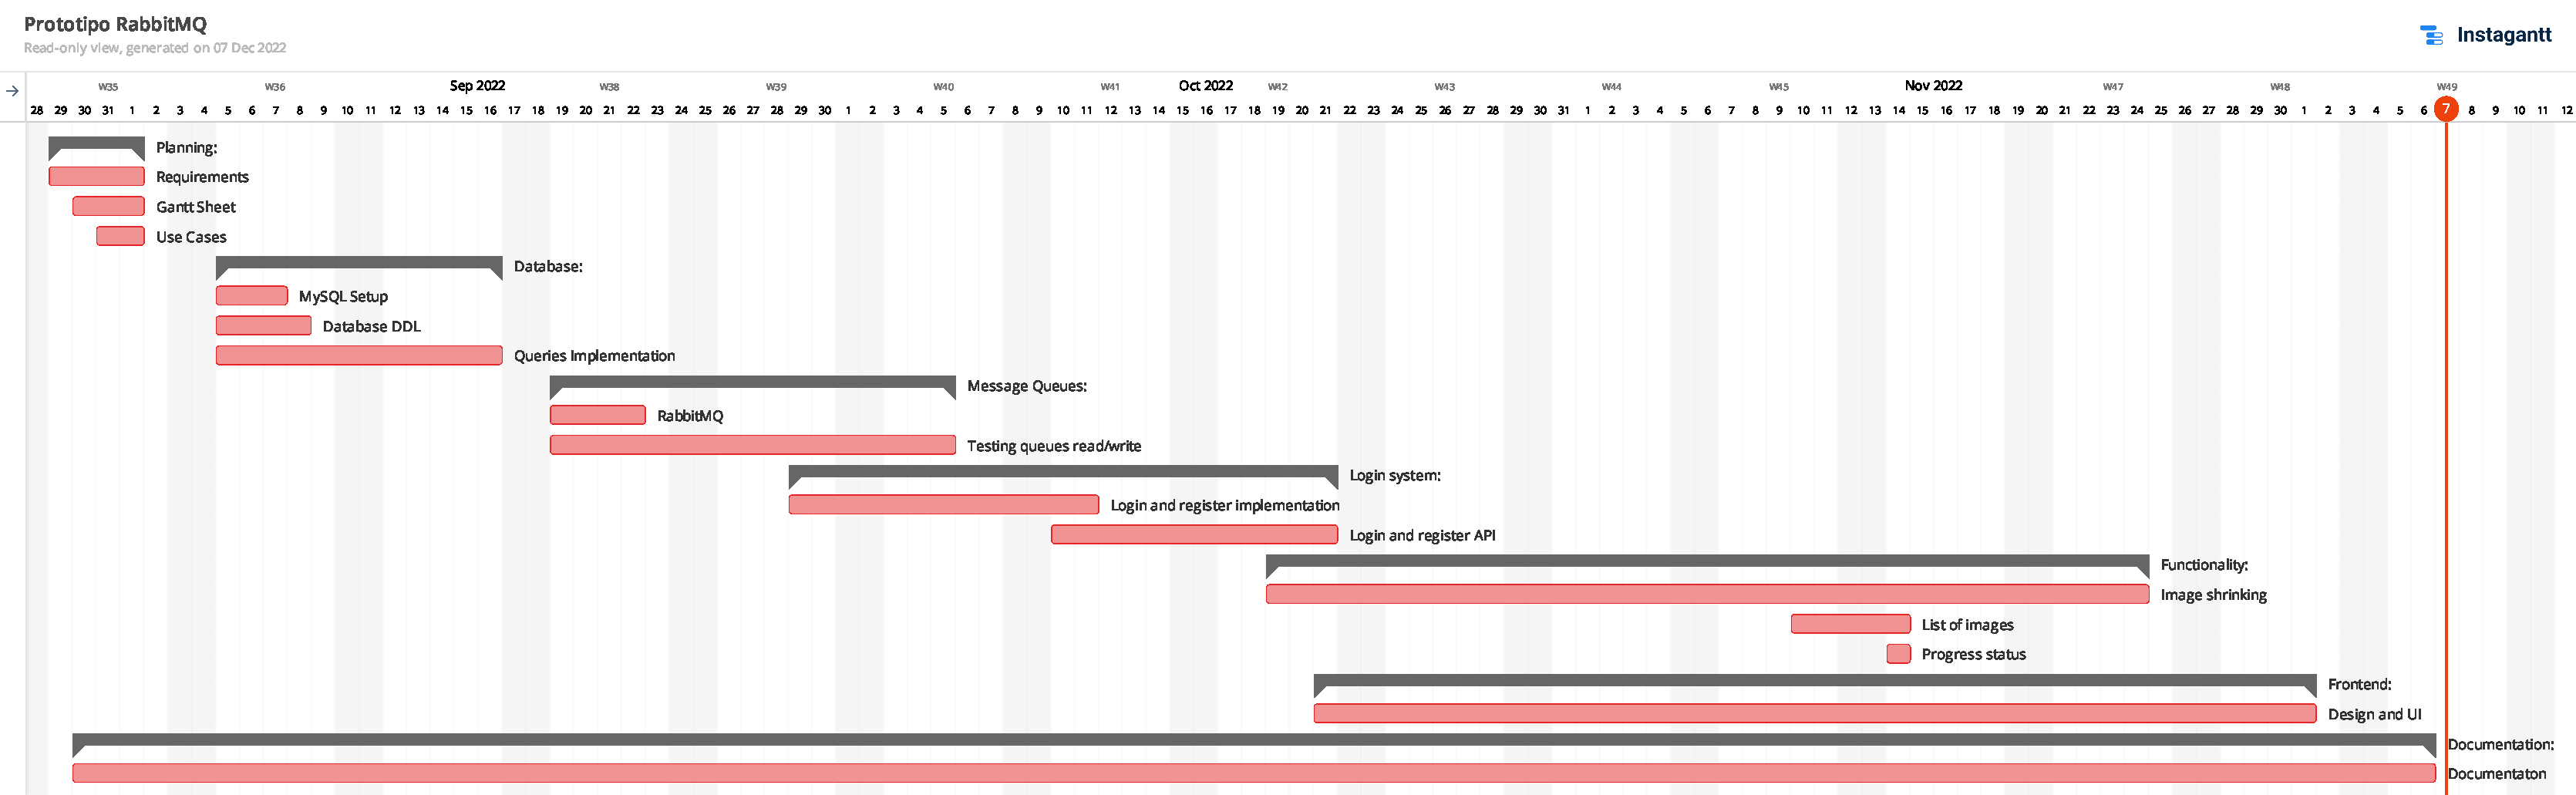
\includegraphics[width=1.3\pagewidth]{gantt2.pdf}}%
    \caption{Final Gantt chart}
\end{figure}

The left side of the initial Gantt chart
has been left as is, whilst in the second half
many tasks have taken longer than expected.

\end{document}